% !TeX program = xelatex

% \documentclass[handout]{beamer}
\documentclass{beamer}
\usepackage[T1]{fontenc}
\usepackage{lmodern}
\usepackage{unicode-latex}
\usepackage{cancel}
\usepackage{hyperref}

\renewcommand\textbullet{\ensuremath{\bullet}}
\newcommand\op{\operatorname}

% Custom title frame
%% https://tex.stackexchange.com/questions/22346/how-to-customize-titlepage-in-beamer
% \titlegraphic{
%   \includegraphics[width=2cm]{kth}
%   
\includegraphics[width=2cm]{su}
% }
 
\beamertemplatenavigationsymbolsempty
\setbeamercolor{title}{fg=black}
\setbeamercolor{frametitle}{fg=black}
\setbeamercolor{framesubtitle}{fg=black}
\setbeamercolor{text}{fg=black}
\setbeamercolor{item}{fg=black}
\setbeamercolor{block title}{fg=black}
\setbeamerfont{block title}{family=\bfseries}


\usepackage{amssymb}
\usepackage{mathbbol}
\DeclareSymbolFontAlphabet{\mathbb}{AMSb}
\DeclareSymbolFontAlphabet{\mathbbl}{bbold}
\newcommand{\bbDelta}{\mathbbl{\Delta}}


\setbeamertemplate{itemize items}[circle]

\usefonttheme{professionalfonts}
% \usepackage{fontspec}
% \setsansfont[Scale=MatchLowercase]{Noto Sans}

% \mode<presentation> { \setbeamercovered{transparent} }
% \makeatletter
% \def\pdftex@driver{pdftex.def}
% \ifx\Gin@driver\pdftex@driver
%   \def\pgfsys@color@unstacked#1{%
%     \pdfliteral{\csname\string\color@#1\endcsname}%
%   }
% \fi
% \makeatother

% \mode<presentation> { \setbeamercovered{transparent} }
% \setbeamertemplate{navigation symbols}{}
% \makeatletter
% \def\beamerorig@set@color{%
%   \pdfliteral{\current@color}%
%   \aftergroup\reset@color
% }
% \def\beamerorig@reset@color{\pdfliteral{\current@color}}
% \makeatother


\newcommand{\centermath}[1]{\par\centerline{\begin{minipage}{\linewidth}#1\end{minipage}}\par}


\usepackage{tikz}
\usepackage{braids}
\usepackage{xifthen}

\makeatletter

\newcounter{mycounter}

\newcommand{\fs}[3][]{
  \begin{tikzpicture}[scale=0.35,font=\footnotesize,anchor=mid,baseline={([yshift=-.5ex]current bounding box.center)}]
    \def\height{1.5}
    \def\offset{0.5}
    \ifthenelse{\equal{#1}{}}{\def\height{1}}{} % Smaller height if no braiding
    \setcounter{mycounter}{0}
    \@for\el:=#2\do{
      \ifthenelse{\equal{#1}{\value{mycounter}}}{
        \braid at (\value{mycounter},\height) s_1^{-1};
        \stepcounter{mycounter}
      }{
        \stepcounter{mycounter}
        \ifthenelse{\equal{#1}{\value{mycounter}}}{
        }{
          \draw (\value{mycounter}, \height) to (\value{mycounter}, 0);
        }
      }
      \node at (\value{mycounter}, \height+\offset) {$\el$};
    }
    \draw (0, 0) to (\value{mycounter}+1, 0);
    \setcounter{mycounter}{0}
    \@for\el:=#3\do{
      \node at (\value{mycounter}+0.5, -0.6) {$\el$};
      \stepcounter{mycounter}
    }
  \end{tikzpicture}
}

\newcommand{\fswide}[3][]{
  \begin{tikzpicture}[scale=0.35,font=\footnotesize,anchor=mid,baseline={([yshift=-.5ex]current bounding box.center)}]
    \def\height{1.75}
    \def\offset{0.5}
    \def\widthfactor{2}
    \ifthenelse{\equal{#1}{}}{\def\height{1}}{} % Smaller height if no braiding
    \setcounter{mycounter}{0}
    \@for\el:=#2\do{
      \ifthenelse{\equal{#1}{\value{mycounter}}}{
        \braid[width=\widthfactor cm, height=1.25 cm] at (\widthfactor*\value{mycounter},\height) s_1^{-1};
        \stepcounter{mycounter}
      }{
        \stepcounter{mycounter}
        \ifthenelse{\equal{#1}{\value{mycounter}}}{
        }{
          \draw (\widthfactor*\value{mycounter}, \height) to (\widthfactor*\value{mycounter}, 0);
        }
      }
      \node at (\widthfactor*\value{mycounter}, \height+\offset) {$\el$};
    }
    \draw (0, 0) to (\widthfactor*\value{mycounter}+\widthfactor*1, 0);
    \setcounter{mycounter}{0}
    \@for\el:=#3\do{
      \node at (\widthfactor*\value{mycounter} + \widthfactor*0.5, -0.6) {$\el$};
      \stepcounter{mycounter}
    }
  \end{tikzpicture}
}

\newcommand{\fsfused}[5]{
  \begin{tikzpicture}[scale=0.35,font=\footnotesize,anchor=mid,baseline={([yshift=-.5ex]current bounding box.center)}]
    \def\height{1.75}
    \def\offset{0.5}
    \node at (1, \height+\offset) {$#2$};
    \node at (2, \height+\offset) {$#3$};
    \draw (0.5, 0) to (2.5, 0);
    \draw (1, \height) to [bend left=-30] (1.5, 1);
    \draw (2, \height) to [bend left=30] (1.5, 1);
    \draw (1.5, 1) to (1.5, 0);
    \node at (0.75, -0.6) {$#1$};
    \node at (2.25, -0.6) {$#4$};
    \node at (2, 0.7) {$#5$};
  \end{tikzpicture}
}

\newcommand{\fsfusedbraided}[5]{
  \begin{tikzpicture}[scale=0.35,font=\footnotesize,anchor=mid,baseline={([yshift=-.5ex]current bounding box.center)}]
    \def\height{3}
    \def\offset{0.5}
    \node at (1, \height+\offset) {$#2$};
    \node at (2, \height+\offset) {$#3$};
    \braid at (1, \height) s_1^{-1};
    \draw (0.5, 0) to (2.5, 0);
    \draw (1, 1.5) to [bend left=-30] (1.5, 1);
    \draw (2, 1.5) to [bend left=30] (1.5, 1);
    \draw (1.5, 1) to (1.5, 0);
    \node at (0.5, -0.6) {$#1$};
    \node at (2.5, -0.6) {$#4$};
    \node at (2, 0.7) {$#5$};
  \end{tikzpicture}
}

\makeatother




\setbeamertemplate{footline}[frame number]




\title{Non-Abelian Anyons: Statistical Repulsion and Topological Quantum Computation}
\author{Viktor Qvarfordt}
\institute{KTH Royal Institute of Technology and Stockholm University}
\date{2017-05-23}




\begin{document}





 
\begin{frame}
  \centering
  \huge
  Non-Abelian Anyons \\[0.5em]
  \Large
  Statistical Repulsion and \\
  Topological Quantum Computation \\[1.5em]
  \normalsize
  \textit{Viktor Qvarfordt} \\[1.5em]
  Master's thesis in Mathematics \\[1em]
  \small
  Supervised by \\
  Douglas Lundholm \\[1em]
  KTH Royal Institute of Technology \\
  and Stockholm University \\[1em]
  2017-05-23
\end{frame}






\begin{frame}{Layout}
  \begin{enumerate}
    \pause
    \item Background and motivation
    \pause
    \item Identical quantum particles: Exchange symmetry
    \pause
    \item Statistical repulsion
    \pause
    \item Abstract anyon models
    \pause
    \item Explicit model: Fibonacci anyons
    \pause
    \item Topological quantum computation with Fibonacci anyons
  \end{enumerate}
\end{frame}








\begin{frame}{Background and motivation: \textit{Sketchy}}
  \vspace{1em}
  Wave function, state of two identical quantum particles
  \begin{equation*}
    ψ(x₁, x₂) : ℝ³ × ℝ³ → ℂ
  \end{equation*}
  \pause
  Probability distribution
  \begin{equation*}
    |ψ(x₁, x₂)|²
  \end{equation*}
  \vspace{-1em}
  \pause
  \begin{alignat*}{3}
    & \text{Bosons:}   & \quad ψ(x₂, x₁) &=  ψ(x₁, x₂) && \quad \text{(symmetric)} \\
    & \text{Fermions:} & \quad ψ(x₂, x₁) &= -ψ(x₁, x₂) && \quad \text{(anti-symmetric)}
  \end{alignat*}
  % \pause
  % Fermions: Electrons, protons neutrons, atoms. \\
  % Bosons: Photons (force carriers), atoms.
  \pause
  \begin{equation*}
    ψ(x₁, x₂) : ℝ² × ℝ² → ℂᵏ
  \end{equation*}
  \vspace{-1em}
  \pause
  \begin{alignat*}{3}
    & \text{Abelian anyons:}     & \quad ψ(x₂, x₁) &= e^{iθ} ψ(x₁, x₂), & \quad k = 1 \\
    & \text{Non-abelian anyons:} & \quad ψ(x₂, x₁) &= U ψ(x₁, x₂),      & \quad k > 1
  \end{alignat*}
  \pause
  Originally due to J. M. Leinaas and J. Myrheim in 1977. \\
  Name `anyons' due to F. Wilczek. \\
  \pause
  Hot topic, recent Nobel prize on Topological states of matter.
\end{frame}









\begin{frame}{Identical quantum mechanical particles}
  \pause
  Consider $n$ indistinguishable quantum particles.
  \pause
  Wave function:
  \begin{equation*}
    ψ : 𝒞ₙ → ℂᵏ
  \end{equation*}
  \pause
  Configuration space:
  \begin{equation*}
    𝒞ₙ = 
    \only<-4>{\makebox[0pt][l]{$Mⁿ$}\phantom{\frac{Mⁿ-\bbDeltaₙ}{Sₙ}}}
    \only<5->{\frac{Mⁿ-\bbDeltaₙ}{Sₙ}}
  \end{equation*}
  \pause
  \pause
  Hard-core:
  \begin{equation*}
    \bbDeltaₙ = \{(x₁,…,xₙ) ∈ Mⁿ ∣ ∃\; i≠j \text{ s.t.\ } xᵢ = xⱼ\}
  \end{equation*}
  \pause
  Identifying particle configurations:
  \begin{equation*}
    (…,xⱼ,…,xₖ,…) = (…,xₖ,…,xⱼ,…)
  \end{equation*}
\end{frame}






\begin{frame}{Exchange symmetries}
  \vspace{0.5em}
  Classical exchange: Loops in $𝒞ₙ$. \\
  \pause
  Quantizing the system: Homotopically equivalent loops give the same contribution. \\
  \pause
  Exchange must obey the structure of $π₁(𝒞ₙ)$. \\
  \pause
  \begin{equation*}
    π₁(𝒞ₙ) =
    \begin{cases}
      Sₙ, & M = ℝᵈ, d ≥ 3, \\
      Bₙ, & M = ℝ².
    \end{cases}
  \end{equation*}
  \pause
  Exchange determined by a unitary representation
  \begin{equation*}
    ρ : π₁(𝒞ₙ) → U(k).
  \end{equation*}
  \pause
  Exchange performs $ψ ↦ Uψ$, s.t.
  \begin{equation*}
    ‖ψ‖² = ‖Uψ‖².
  \end{equation*}
  % \pause
  % Selection rules for observables,
  % \begin{equation*}
  %   ⟨ψ|A|ψ⟩ = ⟨ψ|U^*AU|ψ⟩.
  % \end{equation*}
\end{frame}





\begin{frame}{Braid group $Bₙ$}
  Generators $σ₁, …, σ_{n-1}: \quad$
  \begin{tikzpicture}[scale=0.9,font=\tiny,anchor=mid,baseline={([yshift=0ex]current bounding box.center)}]
    \draw (-0.5, 0) -- (-0.5, -1.5);
    \braid[number of strands=4] at s_2^{-1};
    \node at (-0.5, -1.75) {$1$};
    \node at (0.25, -0.875) {$⋯$};
    \node at (1, -1.75) {$j{-}1$};
    \node at (2, -1.75) {$j$};
    \node at (3, -1.75) {$j{+}1$};
    \node at (4, -1.75) {$j{+}2$};
    \node at (4.75, -0.875) {$⋯$};
    \node at (5.5, -1.75) {$n$};
    \draw (5.5, 0) -- (5.5, -1.5);
    \node at (2.5, -1) {$σⱼ$};
  \end{tikzpicture}\\
  \pause
  Relations
  \begin{align*}
    σⱼ σₖ &= σₖ σⱼ, \quad\text{if } |j-k| ≥ 2, \\
    σⱼ σ_{j+1} σⱼ &= σ_{j+1} σⱼ σ_{j+1} \\
    σⱼ² &= 1 \quad\text{for the symmetric group}
  \end{align*}
  \pause
  \begin{minipage}[c][0.35\textheight][c]{\textwidth}
  \centering
  \only<3>{
  \begin{equation*}
    \begin{tikzpicture}[scale=0.8,font=\tiny,anchor=mid,baseline={([yshift=0ex]current bounding box.center)}]
      \braid[number of strands=6] s_4^{-1}s_2^{-1};
      \node at (1, -2.75) {$j{-}1$};
      \node at (2, -2.75) {$j$};
      \node at (3, -2.75) {$j{+}1$};
      \node at (4, -2.75) {$j{+}2$};
      \node at (5, -2.75) {$j{+}3$};
      \node at (6, -2.75) {$j{+}4$};
      \node at (2.5, -2) {$σⱼ$};
      \node at (4.5, -1) {$σ_{j+2}$};
    \end{tikzpicture}
    {\;}={\;}
    \begin{tikzpicture}[scale=0.8,font=\tiny,anchor=mid,baseline={([yshift=0ex]current bounding box.center)}]
      \braid[number of strands=6] s_2^{-1}s_4^{-1};
      \node at (1, -2.75) {$j{-}1$};
      \node at (2, -2.75) {$j$};
      \node at (3, -2.75) {$j{+}1$};
      \node at (4, -2.75) {$j{+}2$};
      \node at (5, -2.75) {$j{+}3$};
      \node at (6, -2.75) {$j{+}4$};
      \node at (2.5, -1) {$σ_{j}$};
      \node at (4.5, -2) {$σ_{j+2}$};
    \end{tikzpicture}
  \end{equation*}}
  \only<4>{
  \begin{equation*}
    \begin{tikzpicture}[scale=0.9,font=\tiny,anchor=mid,baseline={([yshift=-.5ex]current bounding box.center)}]
      \braid s_1^{-1} s_2^{-1} s_1^{-1};
      \node at (1, -3.75) {$j$};
      \node at (2, -3.75) {$j+1$};
      \node at (3, -3.75) {$j+2$};
      \node at (1.5, -3) {$σ_{j}$};
      \node at (2.5, -2) {$σ_{j+1}$};
      \node at (1.5, -1) {$σ_{j}$};
    \end{tikzpicture}
    {\quad}={\quad}
    \begin{tikzpicture}[scale=0.9,font=\tiny,anchor=mid,baseline={([yshift=-.5ex]current bounding box.center)}]
      \braid s_2^{-1} s_1^{-1} s_2^{-1};
      \node at (1, -3.75) {$j$};
      \node at (2, -3.75) {$j+1$};
      \node at (3, -3.75) {$j+2$};
      \node at (2.5, -3) {$σ_{j+1}$};
      \node at (1.5, -2) {$σ_{j}$};
      \node at (2.5, -1) {$σ_{j+1}$};
    \end{tikzpicture}
  \end{equation*}}
  \end{minipage}
\end{frame}






\begin{frame}{Representations of $π₁(𝒞ₙ)$}
  \pause
  One-dimensional representations of $Sₙ$:
  \begin{alignat*}{3}
    & ρ(σⱼ) = 1  \quad && \text{(bosons)} \\
    & ρ(σⱼ) = -1 \quad && \text{(fermions)}
  \end{alignat*}
  \pause
  Representations of $Bₙ$:
  \begin{alignat*}{3}
    & ρ(σⱼ) = e^{iθ}    \quad && \text{(abelian anyons)} \\
    & ρ(σⱼ) = Uⱼ ∈ U(k) \quad && \text{(non-abelian anyons)}
  \end{alignat*}
  \vspace{-1em}
  \pause
  \begin{align*}
    \text{\textrm{``}}ψ(x₂, x₁) &= U₁ ψ(x₁, x₂)\text{\textrm{''}} \\[1em]
    σ₁ψ(x₁, x₂)     &= U₁ ψ(x₁, x₂)
  \end{align*}
\end{frame}








\begin{frame}{Statistical repulsion: Introduction}
  \vspace{1em}
  Quantum state $ψ(x₁,x₂)$ of two fermions:
  \[ ψ(x₁,x₂) = -ψ(x₂,x₁) \]
  Then $ψ(x,x) = 0$; an instance of the Pauli exclusion principle.

  \pause
  Gives rise to an effective repulsion, statistical repulsion. \\
  Kinetic energy operator: $\widehat{T} = -∇²$.
  \begin{theorem}[Many-body Hardy inequality for fermions]
    \vspace{-1.5em}
    \begin{gather*}
      ⟨ψ|\widehat{T}|ψ⟩ = ∫_{ℝ^{dn}} ∑_{j=1}^n |∇ⱼψ|^2 dx ≥ \\
      ≥ \frac{d²}{n} ∫_{ℝ^{dn}} ∑_{1≤j<k≤n} \frac{|ψ|^2}{|xⱼ-xₖ|^2} dx +
      \frac{1}{n} ∫_{ℝ^{dn}} \left|∑_{j=1}^n ∇ⱼ ψ \right|^2 dx.
    \end{gather*}
  \end{theorem}
\end{frame}







\begin{frame}{Statistical repulsion: Towards anyons}
  Split the sum,
  \vspace{-1em}
  \begin{equation*}
    ∑_{j=1}^n |∇ⱼ ψ|^2 = \frac{1}{n} ∑_{1 \le j < k \le n} \left| (∇ⱼ - ∇ₖ) ψ \right|^2 + \frac{1}{n} \left| ∑_{j=1}^n ∇ⱼ ψ \right|².
  \end{equation*}
  \pause
  Relative coordinates:
  \begin{align*}
    x_\text{rel} &≔ (xⱼ - xₖ)/2, &
    x_\text{cm}  &≔ (xⱼ + xₖ)/2, &
    ∇_\text{rel} &≔ ∇ⱼ - ∇ₖ.
  \end{align*}
  \vspace{-1em}
  \pause
  \begin{equation*}
    ∫_{ℝ^{2n}} \left|(∇ⱼ-∇ₖ)ψ\right|^2 dx
    = ∫_{ℝ^{2(n-2)}} ∫_{ℝ²×ℝ²} \left|∇_\text{rel} ψ\right|^2  2\,dx_\text{rel}\,dx_\text{cm}\,dx'.
  \end{equation*}
  \pause
  Polar coordinates $x_\text{rel} = (r, φ)$,
  \begin{equation*}
    ∫_{ℝ²} \left|∇_\text{rel} ψ\right|^2  dx_\text{rel} =
    ∫_{r=0}^∞ ∫_{φ=0}^{2π} \left( \left|∂ᵣ ψ\right|^2 + \frac{\textcolor{red}{\left|∂_φ ψ\right|²}}{r²} \right) r\,dφ\,dr.
  \end{equation*}
\end{frame}









\begin{frame}{Statistical repulsion: Anyons}
  \begin{equation*}
    ∫₀^π |∂_φ ψ|² dφ \pause = \inf \{ λ² : e^{iλπ} \text{ is an eigenvalue of } Uᵣ \} ≕ λ_{0,r}²
  \end{equation*}
  for anyonic exchange $ψ(π) = Uᵣ ψ(0)$.
  \pause
  \begin{center}
    \includegraphics{img/exchange_loop_p.pdf}
  \end{center}
  \begin{equation*}
    Uₚ = Uᵣ, \quad r_{p-1} < r < rₚ
  \end{equation*}
  \pause
  \begin{equation*}
    Uₚ = ρ(σ₁σ₂⋯σₚσ_{p+1}σₚ⋯σ₂σ₁)
  \end{equation*}
\end{frame}








\begin{frame}{Statistical repulsion: Abelian anyons}
  Same exchange for all generators:
  \begin{equation*}
    ρ(σⱼ) = e^{iαπ} \quad\text{for all $j$}
  \end{equation*}
  \vspace*{-1em}
  \pause
  \begin{equation*}
    Uₚ = ρ(σ₁σ₂⋯σₚσ_{p+1}σₚ⋯σ₂σ₁) = e^{i(2p+1)απ}
  \end{equation*}
  \pause
  \begin{equation*}
    λ_{0,p}² = \left\{ λ² : e^{iλπ} \text{ is an eigenvalue of } Uₚ \right\} = \min_{q ∈ ℤ} \left\{ \big((2p+1)α + 2q\big)² \right\}
  \end{equation*}
  \pause
  \begin{alignat*}{3}
      \text{Bosons ($α = 0$):} & \quad Uₚ = 1  = e^{i0} & ⟹ λ_{0,p}² = 0. \\
    \text{Fermions ($α = 1$):} & \quad Uₚ = -1 = e^{iπ} & ⟹ λ_{0,p}² = 1.
  \end{alignat*}
  Both independent of $p$.
  
  \pause
  Difficult to characterize $Uₚ$ generally.
\end{frame}









\begin{frame}{Abstract anyon models}
  \pause
  \textit{Formally described by modular tensor categories, encoding the topological structure of 2D conformal field theories.}
  \\[1em]
  \pause
  Introducing an interaction: Fusion. \\
  \pause
  Fusion algebra: A set of labels $\{a,b,c,…\}$ and fusion rules:
  \begin{equation*}
    a × b = ∑_c N_{ab}^c c
  \end{equation*}
  \pause
  Fusion diagrams:
  \begin{equation*}
    \begin{array}{r@{}l}
      \fswide{a₂}{a₁,c} &{}⟺ a₁ × a₂ = c \\
      \pause
      \fswide{a₂,a₃}{a₁,b₁,c} &{}⟺ \underbrace{a₁ × a₂}_{b₁} × a₃ = c \\
      \pause
      \fswide{a₂,a₃,a₄}{a₁,b₁,b₂,c} &{}⟺ \underbrace{\underbrace{a₁ × a₂}_{b₁} × a₃}_{b₂} × a₄ = c
    \end{array}
  \end{equation*}
\end{frame}







\begin{frame}{Abstract anyon models: Fusion spaces}
  Fusion spaces: $V_{a₁⋯aₙ}^c$ is the Hilbert space of all possible fusion states s.t.
  \[ a₁ × ⋯ × aₙ = c. \]
  \pause
  Canonical decomposition:
  \begin{equation*}
    V_{a_1 \cdots a_n}^c \cong \bigoplus_{b_1,b_2,\ldots,b_{n-2}} V_{a_1a_2}^{b_1} \otimes V_{b_1 a_3}^{b_2} \otimes V_{b_2 a_4}^{b_3} \ldots \otimes V_{b_{n-2} a_n}^c
  \end{equation*}
  \pause
  Standard basis for $V_{a₁⋯aₙ}^c$:
  \begin{equation*}
    \left\{
    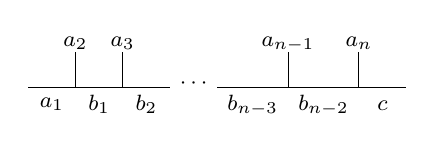
\begin{tikzpicture}[scale=0.3,font=\footnotesize,anchor=mid,baseline={([yshift=-.5ex]current bounding box.center)}]
      \node at (0, -0.6) {$a_1$};
      \node at (1, 2) {$a_2$};
      \node at (3, 2) {$a_3$};
      \node at (10, 2) {$a_{n-1}$};
      \node at (13, 2) {$a_n$};
  %
      \draw (1, 0) to (1, 1.5);
      \draw (3, 0) to (3, 1.5);
  %
      \draw (10, 0) to (10, 1.5);
      \draw (13, 0) to (13, 1.5);
  %
      \draw (-1, 0) to (5, 0);
      \draw (7, 0) to (15, 0);
  %
      \node at (2, -0.7) {$b_1$};
      \node at (4, -0.7) {$b_2$};
      \node at (6, 0.2) {$\cdots$};
  %
      \node at (8.5, -0.7) {$b_{n-3}$};
      \node at (11.5, -0.7) {$b_{n-2}$};
      \node at (14, -0.7) {$c$};
    \end{tikzpicture}
    \;\;\;\bigg|\; \begin{array}{c}\text{for all possible intermediate} \\ \text{charges $b_1, b_2, \ldots, b_{n-2}$}\end{array}
    \right\}
  \end{equation*}
  % For given anyons $a_1, \ldots, a_n$ the fusion states are determined by the intermediate charges $b_j$.
\end{frame}







\begin{frame}{Abstract anyon models: Fusion}
  Associativity of fusion:
  \begin{equation*}
    (a \times b) \times c = a \times (b \times c)
  \end{equation*}
  \pause
  Natural isomorphism:
  \begin{equation*}
    \begin{array}{r@{}l@{}c@{}l@{}c}
      V_{abc}^d \cong{} & \displaystyle\bigoplus_f {} & V_{ab}^f \otimes V_{fc}^d & {} \cong \displaystyle\bigoplus_e {} &V_{bc}^e \otimes V_{ea}^d \\
      \pause
                \iff {} & \displaystyle\bigoplus_f    & \fs{b,c}{a,f,d}           & {} \cong \displaystyle\bigoplus_e {} &\fsfused{a}{b}{c}{d}{e}
    \end{array}
  \end{equation*}
  \pause
  This isomorphism is given by the $F$ operator:
  \begin{equation*}
    F_{abc}^d : \fs{b,c}{a,e,d} \mapsto \fsfused{a}{b}{c}{d}{e} = \sum_f \left(F_{abc}^d\right)_{fe} \fs{b,c}{a,f,d}
  \end{equation*}
\end{frame}







\begin{frame}{Abstract anyon models: Braiding}
  The $R$ operator: Isomorphism $R_{ab}^c : V_{ab}^c → V_{ba}^c$:
  \vspace{-0.5em}
  \begin{equation*}
    R_{ab} : \fsfused{}{a}{b}{}{c} \mapsto \fsfusedbraided{}{a}{b}{}{c} = R_{ab}^c \fsfused{}{a}{b}{}{c}
    \vspace{-1.5em}
  \end{equation*}
  \pause
  Define the $B$ operator in terms of the $F$ and $R$ operator:
  \begin{equation*}
    \left(B_{abc}^d\right)_{eg} = \sum_f \left(\left(F^{-1}\right)_{acb}^d\right)_{fe} R_{bc}^f \left(F_{abc}^d\right)_{gf}.
  \end{equation*}
  \pause
  Braiding on standard fusion states:
  \begin{equation*}
    B_{abc}^d : \fs{b,c}{a,e,d} \mapsto \fs[1]{b,c}{a,e,d} = \sum_g \left(B_{abc}^d\right)_{ge} \fs{b,c}{a,g,d}
  \end{equation*}
  \pause
  Symbolically: $B = F^{-1} R F$. Representation of $Bₙ$.
\end{frame}







\begin{frame}{Abstract anyon models: Consistency: Pentagon equation}
  \centering
  \includegraphics[width=\textwidth]{img/pentagon_diagram.pdf}
\end{frame}

\begin{frame}{Abstract anyon models: Consistency: Hexagon equation}
  \centering
  \vspace{1em}
  \includegraphics[width=0.9\textwidth]{img/hexagon_diagram.pdf}
\end{frame}







\begin{frame}{Abstract anyon models: Exchange operator $Uₚ$}
  \pause
  \vspace{1em}
  Non-trivial charge label $t$, fusion space $V_{t^{p+2}}$.
  \vspace{-1em}
  \begin{equation*}
    \begin{tikzpicture}[scale=0.2,font=\footnotesize,anchor=mid]
      \draw (-27, -1) to (-27, -3); % vertical
      \node at (-27, 0) {$t$};
      \draw (-24, -1) to (-24, -3); % vertical
      \node at (-24, 0) {$t$};
      \node at (-21, -1.5) {$\cdots$};
      \draw (-18, -1) to (-18, -3); % vertical
      \node at (-18, 0) {$t$};
      \draw (-15, -1) to (-15, -3); % vertical
      \node at (-15, 0) {$t$};
      \draw (-30, -3) to (-12, -3); % horizontal
      \node[font=\large] at (-8, -1.5) {$\xmapsto{\;\;F\;\;}$};
      \draw (2, 6) to [bend left=-30] (3, 4);
      \draw (4, 6) to [bend left=30]  (3, 4);
      \draw (1, 4) to [bend left=-30] (2, 2);
      \draw (3, 4) to [bend left=30]  (2, 2);
      \draw (0, 2) to [bend left=-30] (1, 0);
      \draw (2, 2) to [bend left=30]  (1, 0);
      \draw (1, 0) to (1, -3); % vertical under bend
      \node at (1+0.75, -0.75) {$c$};
      \node[font=\scriptsize] at (3.4, 1.4) {$c_1$};
      \node[font=\scriptsize] at (4.4, 3.4) {$c_2$};
      \node[font=\scriptsize] at (5.4, 5.4) {$c_3$};
      \node at (0, 2+1) {$t$};
      \node at (1, 4+1) {$t$};
      \node at (2, 6+1) {$t$};
      \node[rotate=-20] at (4.25, 6+1.25) {$\vdots$};
      \draw (-5, -3) to (7, -3); % horizontal
      \draw (-2.5, 0) to (-2.5, -3); % vertical left of bend
      \draw (4.5, 0) to (4.5, -3); % vertical right of bend
      \node at (-2.5+0.75, -0.75) {$t$};
      \node at (4.5+0.75, -0.75) {$t$};
      %
      \node[font=\normalsize] at (11, -1.5) {$\eqqcolon$};
      \draw (17, -1) to (17, -3); % vertical
      \draw (20, -1) to (20, -3); % vertical
      \draw (23, -1) to (23, -3); % vertical
      \node at (17, 0) {$t$};
      \node at (20, 0) {$c$};
      \node at (23, 0) {$t$};
      \draw (15, -3) to (25, -3); % horizontal
    \end{tikzpicture}
  \end{equation*}
  \pause
  Gives rise to the decomposition:
  \begin{equation*}
    V_{t^{p+2}} = ⨁_c V_{t^p}^c ⊗ V_{tct}
  \end{equation*}
  \vspace{-0.75cm}
  \pause
  \begin{theorem}
    The exchange operator is given by $\displaystyle U_p = \bigoplus_{c} U_{1,c}$ where
    % where $U_{1,c}$ denotes the exchange operator for two $t$ anyons around one anyon of type $c$, and $c$ ranges over all possible total charges of the $p$ enclosed anyons, that is, the possible total charges $c$ for the fusion space $V_{t^p}^c$. $U_{1,c}$ is given by
    % \centermath{
    \vspace{-1em}
    \small
    \begin{equation*}
      \begin{aligned}
        U_{1,c} \left( \fs{t,c,t}{a,b,d,e} \right) =
        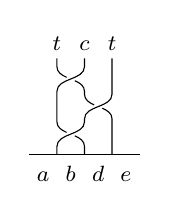
\begin{tikzpicture}[scale=0.35,font=\footnotesize,anchor=mid,baseline={([yshift=-.5ex]current bounding box.center)}]
          \braid s_1^{-1} s_2^{-1} s_1^{-1};
          \node at (1, 0.5) {$t$};
          \node at (2, 0.5) {$c$};
          \node at (3, 0.5) {$t$};
          \draw (0, -3.5) to (4, -3.5);
          \node at (0.5, -4.25) {$a$};
          \node at (1.5, -4.25) {$b$};
          \node at (2.5, -4.25) {$d$};
          \node at (3.5, -4.25) {$e$};
        \end{tikzpicture} =
        \underbrace{\sum_{f,g,h} \left( B_{act}^d \right)_{fb} \left( B_{ftt}^e \right)_{gd} \left( B_{at c}^g \right)_{hf}}_{ρ(σ₁σ₂σ₁)}
        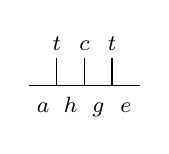
\begin{tikzpicture}[scale=0.35,font=\footnotesize,anchor=mid,baseline={([yshift=-.5ex]current bounding box.center)}]
          \draw (1, 0) to (1, -1);
          \draw (2, 0) to (2, -1);
          \draw (3, 0) to (3, -1);
          \node at (1, 0.5) {$t$};
          \node at (2, 0.5) {$c$};
          \node at (3, 0.5) {$t$};
          \draw (0, -1) to (4, -1);
          \node at (0.5, -1.75) {$a$};
          \node at (1.5, -1.75) {$h$};
          \node at (2.5, -1.75) {$g$};
          \node at (3.5, -1.75) {$e$};
        \end{tikzpicture}.
      \end{aligned}
    \end{equation*}
    % }
  \end{theorem}
\end{frame}







\begin{frame}{Fibonacci anyons}
  \pause
  Two charge labels:
  \begin{itemize}
    \item $1$ (trivial, vacuum)
    \item $τ$ (the Fibonacci anyon)
  \end{itemize}
  \pause
  Fusion rules:
  \begin{equation*}
    \begin{array}{r@{}l}
      1 × 1 &{}= 1 \\
      1 × τ &{}= τ \\
      τ × 1 &{}= τ \\
      τ × τ &{}= 1 + τ \\
      \pause
      τ × τ × τ &{}= 1 + 2⋅τ \\
      \pause
      τ×τ×τ×τ &{}= 2⋅1 + 3⋅τ \\
      \pause
      τ^n &{}= \op{Fib}(n-1)⋅1 + \op{Fib}(n)⋅τ
    \end{array}
  \end{equation*}
  \centering
  \renewcommand{\arraystretch}{1.2}
  \begin{tabular}{c|ccccccccccc}
    $n$           & $0$ & $1$ & $2$ & $3$ & $4$ & $5$ & $6$ & $7$  & $⋯$ \\ \hline
    $\op{Fib}(n)$ & $0$ & $1$ & $1$ & $2$ & $3$ & $5$ & $8$ & $13$ & $⋯$ 
  \end{tabular}
\end{frame}






\begin{frame}{Fibonacci anyons: Solving the model}
  Solving the Pentagon and Hexagon equations gives
  \begin{equation*}
    \begin{array}{r @{{}={}} c @{{}={}} c}
      F_{τττ}^τ &
      \begin{pmatrix}
        \left(F_{τττ}^τ\right)_{11} & \left(F_{τττ}^τ\right)_{1τ} \\[0.5em]
        \left(F_{τττ}^τ\right)_{τ1} & \left(F_{τττ}^τ\right)_{ττ}
      \end{pmatrix}
      &
      \begin{pmatrix}
        φ^{-1} & φ^{-1/2} \\[0.5em]
        φ^{-1/2} & -φ^{-1}
      \end{pmatrix} \\[1em]
      R_{ττ} &
      \begin{pmatrix}
        R_{ττ}^1 & 0 \\[0.5em]
        0 & R_{ττ}^τ
      \end{pmatrix}
      &
      \begin{pmatrix}
        e^{4π i/5} & 0 \\[0.5em]
        0 & e^{-3π i/5}
      \end{pmatrix}
    \end{array}
  \end{equation*}
  as the only non-trivial instances of the $F$ and $R$ matrices, \pause where
  \[ φ = \lim_{n → ∞} \frac{\op{Fib}(n)}{\op{Fib}(n-1)} = \frac{1+√5}{2} \]
  is the golden ratio.
  % \pause
  % Let
  % \begin{equation*}
  %   \begin{aligned}
  %     F \coloneqq F_{τττ}^τ, &&
  %     R \coloneqq R_{ττ}, &&
  %     B \coloneqq F^{-1} R F.
  %   \end{aligned}
  % \end{equation*}
\end{frame}








\begin{frame}{Fibonacci anyons: $Uₚ$ and statistical repulsion}
  \pause
  \small
  \begin{equation*}
    Uₚ = ⨁_c U_{1,c} = U_{1,1} ⊕ U_{1,τ}
  \end{equation*}
  \vspace{-0.5em}
  \begin{equation*}
    \begin{aligned}
      U_{1,c} \left( \fs{t,c,t}{a,b,d,e} \right) =
      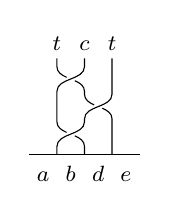
\begin{tikzpicture}[scale=0.35,font=\footnotesize,anchor=mid,baseline={([yshift=-.5ex]current bounding box.center)}]
        \braid s_1^{-1} s_2^{-1} s_1^{-1};
        \node at (1, 0.5) {$t$};
        \node at (2, 0.5) {$c$};
        \node at (3, 0.5) {$t$};
        \draw (0, -3.5) to (4, -3.5);
        \node at (0.5, -4.25) {$a$};
        \node at (1.5, -4.25) {$b$};
        \node at (2.5, -4.25) {$d$};
        \node at (3.5, -4.25) {$e$};
      \end{tikzpicture} =
      ρ(σ₁σ₂σ₁)
      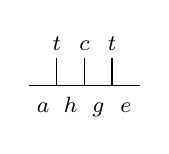
\begin{tikzpicture}[scale=0.35,font=\footnotesize,anchor=mid,baseline={([yshift=-.5ex]current bounding box.center)}]
        \draw (1, 0) to (1, -1);
        \draw (2, 0) to (2, -1);
        \draw (3, 0) to (3, -1);
        \node at (1, 0.5) {$t$};
        \node at (2, 0.5) {$c$};
        \node at (3, 0.5) {$t$};
        \draw (0, -1) to (4, -1);
        \node at (0.5, -1.75) {$a$};
        \node at (1.5, -1.75) {$h$};
        \node at (2.5, -1.75) {$g$};
        \node at (3.5, -1.75) {$e$};
      \end{tikzpicture}.
    \end{aligned}
  \end{equation*}
  \pause
  \vspace{-1em}
  \begin{theorem}
    \vspace{-0.5em}
    \begin{minipage}{0.5\textwidth}
      \begin{align*}
        U₀ &= U_{1,1} \quad  U₁ = U_{1,τ} \\
        Uₚ &= U₀^{⊕\op{Fib}(p-1)} ⊕ U₁^{⊕\op{Fib}(p)}, \quad p ≥ 2
      \end{align*}
      \footnotesize
      \vspace{-1em}
      \pause
      \begin{equation*}
        \sigma(U_p) =
        \left\{
        \begin{array}{rl}
          e^{i4π/5}  &\text{\rm mult. }\,\; \phantom{2}\op{Fib}(p+3), \\
          e^{iπ/5}   &\text{\rm mult. }\,\; 2\op{Fib}(p), \\
          e^{-iπ/5}  &\text{\rm mult. }\,\; 3\op{Fib}(p), \\
          e^{-i3π/5} &\text{\rm mult. }\,\; 3\op{Fib}(p-1)
        \end{array}
        \right\},
      \end{equation*}
    \end{minipage}%
    \begin{minipage}[r]{0.5\textwidth}
      \pause
      \hfill\begin{tikzpicture}[scale=1.3]
        \draw[->] (-1.25,0) -- (1.25,0) node[below] {\normalfont\textrm{Re}};
        \draw[->] (0,-1.25) -- (0,1.25) node[right] {\normalfont\textrm{Im}};
        \draw (0,0) circle (1);
        \node[font=\large] at ({cos(deg(pi/5))}, {sin(deg(pi/5))}) {$\bullet$};
        \node at ({cos(deg(pi/5))+0.4}, {sin(deg(pi/5))+0.15}) {$e^{iπ/5}$};
        \node[font=\large] at ({cos(-deg(pi/5))}, {sin(-deg(pi/5))}) {$\bullet$};
        \node at ({cos(-deg(pi/5))+0.3}, {sin(-deg(pi/5))-0.15}) {$e^{-iπ/5}$};
        \node[font=\large] at ({cos(deg(4*pi/5))}, {sin(deg(4*pi/5))}) {$\bullet$};
        \node at ({cos(deg(4*pi/5))-0.3}, {sin(deg(4*pi/5))+0.15}) {$e^{i4π /5}$};
        \node[font=\large] at ({cos(-deg(3*pi/5))}, {sin(-deg(3*pi/5))}) {$\bullet$};
        \node at ({cos(-deg(3*pi/5))-0.15}, {sin(-deg(3*pi/5))-0.25}) {$e^{-3iπ/5}$};
      \end{tikzpicture}
    \end{minipage}
    \pause
    \begin{equation*}
      \text{Statistical repulsion:}\quadλ_{0,0}² = (3/5)², \quad λ_{0,p}² = (1/5)² \text{ for $p≥1$.}
    \end{equation*}
  \end{theorem}
\end{frame}








\begin{frame}{Topological quantum computation with Fibonacci anyons}
  \pause
  \vspace{0.5em}
  Qubit $∈ \op{span}\Big\{|0⟩ + |1⟩\Big\} = ℂ²$ with some identifications.
  \pause

  Observe that $\op{dim} \left(V_{τ^4}^1\right) = 2$, since
  \begin{equation*}
    τ×τ×τ×τ = τ×τ×(1+τ) = τ×(1 + 2⋅τ) = 2⋅1 + \cancel{3⋅τ}.
  \end{equation*}
  \pause
  Define the computational basis as
  \begin{equation*}
    |0⟩ ≔ \fs{τ,τ,τ,τ}{1,τ,1,τ,1}, \quad
    |1⟩ ≔ \fs{τ,τ,τ,τ}{1,τ,τ,τ,1}.
  \end{equation*}
  \pause
  Braid group generators
  \small
  \begin{align*}
    ρ(σ_1) & : \fs{τ,τ,τ,τ}{,,b,,} ↦ \fs[1]{τ,τ,τ,τ}{,,b,,}, \\[-0.5em]
    ρ(σ_2) & : \fs{τ,τ,τ,τ}{,,b,,} ↦ \fs[2]{τ,τ,τ,τ}{,,1,,} + \fs[2]{τ,τ,τ,τ}{,,τ,,}, \\[-0.5em]
    ρ(σ_3) & : \fs{τ,τ,τ,τ}{,,b,,} ↦ \fs[3]{τ,τ,τ,τ}{,,b,,}.
  \end{align*}
\end{frame}









\begin{frame}{Topological quantum computation with Fibonacci anyons}
  Available manipulations on the Fibonacci qubit
  \begin{align*}
    ρ(σ₁) &= ρ(σ₃) = R =
    \begin{pmatrix}
      e^{4πi/5} & 0 \\
      0 & e^{-3πi/5}
    \end{pmatrix} \\
    ρ(σ₂) &= B = F^{-1} R F =
    \begin{pmatrix}
      φ^{-1} e^{-4πi/5} & φ ^{-1/2} e^{3πi/5} \\
      φ^{-1/2} e^{3πi/5} & -φ^{-1}
    \end{pmatrix}
  \end{align*}
  and their inverses.\\
  \pause
  Universal quantum computation: Quantum qubit gates are elements of $U(2)$, Fibonacci braid operators are dense in $U(2)$.\\
  \pause
  Multi-qubit systems and entanglement by inter-qubit braiding.\\
  \pause
  Quantum dimension:
  \begin{equation*}
    d_\tau = \lim_{n\to\infty} \frac{\op{dim}\left( V^1_{\tau^{n+1}} \right)}{\op{dim}\left( V^1_{\tau^{n}} \right)}
    = \lim_{n\to\infty} \frac{\op{Fib}(n)}{\op{Fib}(n-1)} = \varphi
  \end{equation*}
  compare to distinguishable particles with $h = ℂᵏ$
  \begin{equation*}
    ℋₙ = h^{⊗n}, \quad d = \frac{\op{dim} ℋ_{n+1}}{\op{dim}ℋ_{n}} = \op{dim} h = k ∈ ℕ.
  \end{equation*}
\end{frame}








\begin{frame}{Summary and conclusion}
  \begin{itemize}
    \pause
    \item Anyons arise as identical quantum mechanical particles in 2 spatial dimensions.
    \pause
    \item Exchange corresponds to braids in 2+1 dimensional spacetime. Exchange symmetry determined by a representation of the braid group.
    \pause
    \item Statistical repulsion: Lower bound for kinetic energy via the spectrum of the exchange operator $U_p$, \[ λ_0^2 = \inf \{ λ^2 : e^{iλπ} ∈ σ(U_p) \}. \] \vspace{-1.5em}
    \pause
    \item Abstract anyon models, fusion and braiding. General characterization of $U_p$.
    \pause
    \item Fibonacci anyons: Explicit results for $U_p$ and statistical repulsion.
    \pause
    \item Universal topological quantum computation with Fibonacci qubits in $V_{τ^4}^1$.
    \pause
    \item \url{viktorq.se/nonabelions.pdf}
  \end{itemize}
\end{frame}






\end{document}
